\documentclass[journal,12pt,twocolumn]{IEEEtran}

\usepackage{setspace}
\usepackage{gensymb}
\singlespacing
\usepackage[cmex10]{amsmath}

\usepackage{amsthm}

\usepackage{mathrsfs}
\usepackage{txfonts}
\usepackage{stfloats}
\usepackage{bm}
\usepackage{cite}
\usepackage{cases}
\usepackage{subfig}

\usepackage{longtable}
\usepackage{multirow}
\usepackage{adjustbox}
\usepackage{enumitem}
\usepackage{mathtools}
\usepackage{steinmetz}
\usepackage{tikz}
\usepackage{circuitikz}
\usepackage{verbatim}
\usepackage{tfrupee}
\usepackage[breaklinks=true]{hyperref}
\usepackage{graphicx}
\usepackage{tkz-euclide}
\usepackage{tikz}
\usetikzlibrary{shapes.multipart}

\usetikzlibrary{calc,math}
\usepackage{listings}
    \usepackage{color}                                            %%
    \usepackage{array}                                            %%
    \usepackage{longtable}                                        %%
    \usepackage{calc}                                             %%
    \usepackage{multirow}                                         %%
    \usepackage{hhline}                                           %%
    \usepackage{ifthen}                                           %%
    \usepackage{lscape}     
\usepackage{multicol}
\usepackage{chngcntr}

\DeclareMathOperator*{\Res}{Res}

\renewcommand\thesection{\arabic{section}}
\renewcommand\thesubsection{\thesection.\arabic{subsection}}
\renewcommand\thesubsubsection{\thesubsection.\arabic{subsubsection}}
% \renewcommand{\thefigure}{\theenumi}
\renewcommand\thesectiondis{\arabic{section}}
\renewcommand\thesubsectiondis{\thesectiondis.\arabic{subsection}}
\renewcommand\thesubsubsectiondis{\thesubsectiondis.\arabic{subsubsection}}
\usepackage{tikz}
\usetikzlibrary{shapes,arrows}

\hyphenation{op-tical net-works semi-conduc-tor}
\def\inputGnumericTable{}                                 %%

\lstset{
%language=C,
frame=single, 
breaklines=true,
columns=fullflexible
}

\begin{document}


\newtheorem{theorem}{Theorem}[section]
\newtheorem{problem}{Problem}
\newtheorem{proposition}{Proposition}[section]
\newtheorem{lemma}{Lemma}[section]
\newtheorem{corollary}[theorem]{Corollary}
\newtheorem{example}{Example}[section]
\newtheorem{definition}[problem]{Definition}

\newcommand{\BEQA}{\begin{eqnarray}}
\newcommand{\EEQA}{\end{eqnarray}}
\newcommand{\define}{\stackrel{\triangle}{=}}
\bibliographystyle{IEEEtran}
\raggedbottom
\setlength{\parindent}{0pt}
\providecommand{\mbf}{\mathbf}
\providecommand{\pr}[1]{\ensuremath{\Pr\left(#1\right)}}
\providecommand{\qfunc}[1]{\ensuremath{Q\left(#1\right)}}
\providecommand{\sbrak}[1]{\ensuremath{{}\left[#1\right]}}
\providecommand{\lsbrak}[1]{\ensuremath{{}\left[#1\right.}}
\providecommand{\rsbrak}[1]{\ensuremath{{}\left.#1\right]}}
\providecommand{\brak}[1]{\ensuremath{\left(#1\right)}}
\providecommand{\lbrak}[1]{\ensuremath{\left(#1\right.}}
\providecommand{\rbrak}[1]{\ensuremath{\left.#1\right)}}
\providecommand{\cbrak}[1]{\ensuremath{\left\{#1\right\}}}
\providecommand{\lcbrak}[1]{\ensuremath{\left\{#1\right.}}
\providecommand{\rcbrak}[1]{\ensuremath{\left.#1\right\}}}
\theoremstyle{remark}
\newtheorem{rem}{Remark}
\newcommand{\sgn}{\mathop{\mathrm{sgn}}}
% \providecommand{\abs}[1]{\left\vert#1\right\vert}
% \providecommand{\res}[1]{\Res\displaylimits_{#1}} 
% \providecommand{\norm}[1]{\left\lVert#1\right\rVert}
% %\providecommand{\norm}[1]{\lVert#1\rVert}
% \providecommand{\mtx}[1]{\mathbf{#1}}
% \providecommand{\mean}[1]{E\left[ #1 \right]}
\providecommand{\fourier}{\overset{\mathcal{F}}{ \rightleftharpoons}}
%\providecommand{\hilbert}{\overset{\mathcal{H}}{ \rightleftharpoons}}
\providecommand{\system}{\overset{\mathcal{H}}{ \longleftrightarrow}}
	%\newcommand{\solution}[2]{\textbf{Solution:}{#1}}
\newcommand{\solution}{\noindent \textbf{Solution: }}
\newcommand{\cosec}{\,\text{cosec}\,}
\providecommand{\dec}[2]{\ensuremath{\overset{#1}{\underset{#2}{\gtrless}}}}
\newcommand{\myvec}[1]{\ensuremath{\begin{pmatrix}#1\end{pmatrix}}}
\newcommand{\mydet}[1]{\ensuremath{\begin{vmatrix}#1\end{vmatrix}}}
\numberwithin{equation}{subsection}
\makeatletter
\@addtoreset{figure}{problem}
\makeatother
\let\StandardTheFigure\thefigure
\let\vec\mathbf
\renewcommand{\thefigure}{\theproblem}
\def\putbox#1#2#3{\makebox[0in][l]{\makebox[#1][l]{}\raisebox{\baselineskip}[0in][0in]{\raisebox{#2}[0in][0in]{#3}}}}
     \def\rightbox#1{\makebox[0in][r]{#1}}
     \def\centbox#1{\makebox[0in]{#1}}
     \def\topbox#1{\raisebox{-\baselineskip}[0in][0in]{#1}}
     \def\midbox#1{\raisebox{-0.5\baselineskip}[0in][0in]{#1}}
\vspace{3cm}



\title{Assignment 1}
\author{Shreekara Raghavan - EE18BTECH11040}
\maketitle
\newpage
\bigskip
\renewcommand{\thefigure}{\theenumi}
\renewcommand{\thetable}{\theenumi}


\section{Problem}
Let T be a full binary tree with 8 leaves. (A full binary tree has every level full.) Suppose two leaves a and b of T are chosen uniformly and independently at random. The expected value of the distance between a and b in T (i.e., the number of edges in the unique path between a and b) is (rounded off to 2 decimal places)



\section{Full Binary Tree}
\begin{itemize}
    \item A full binary tree is a binary tree whose nodes (apart from the leaf nodes) have 2 children.
    \\
    \item If a binary tree has leaf nodes in the form of $ 2^{k}$, then these kinds of binary trees becomes a perfect binary tree whose height is k.
\end{itemize}

\begin{figure}[!h]
    \centering
    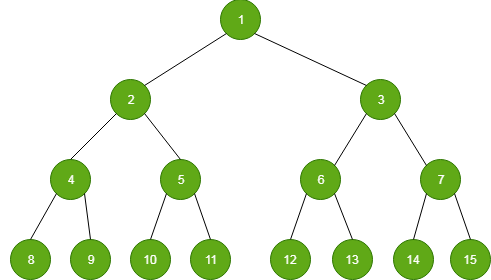
\includegraphics[scale = 0.7]{Perfect-Binary-Tree2.png}
    \caption{Full binary Tree with 8 Leaf Nodes}
    \label{fig:2}
\end{figure}


\section{Distance between 2 Leaf Nodes}

There exists a unique path between 2 nodes of a binary tree without retracing the same edge. The length of the path taken depends on which leaf nodes we choose, specifically at what level their common ancestor is above the leaf nodes. 
\\
\begin{itemize}
    \item If the common ancestor of the leaf nodes(say a and b) is placed 1 level above the leaf node, (the 2 leaf nodes are sibling nodes) then the path length would be 1 ( distance between node a and the parent node) + 1 ( distance between parent node and node b) = 2.
    \begin{figure}[!h]
        \centering
        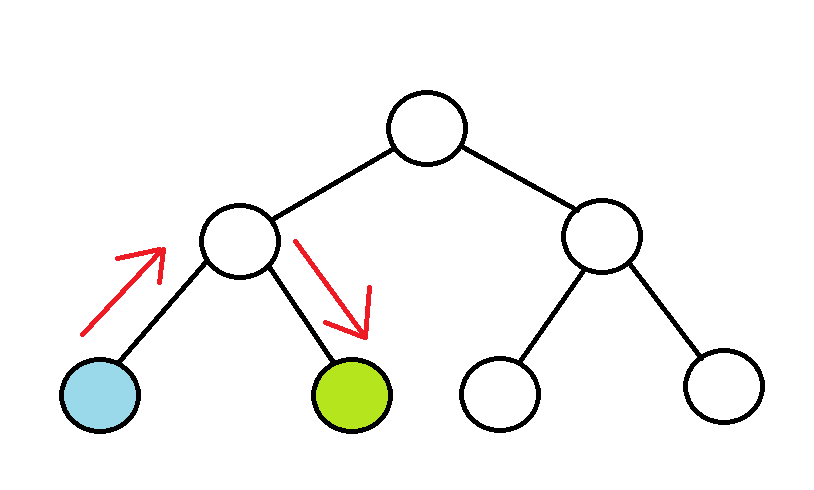
\includegraphics[scale = 0.3]{treea.png}
        \caption{distance when common ancestor is 1 level above = 2}
        \label{fig:2}
    \end{figure}
    \\
    \item Similarly, if If the common ancestor of the leaf nodes is placed 2 levels above the leaf node, then the path length would be 2 ( distance between node a and the common ancestor) + 2 ( distance between common ancestor and node b) = 4.
    \begin{figure}[!h]
        \centering
        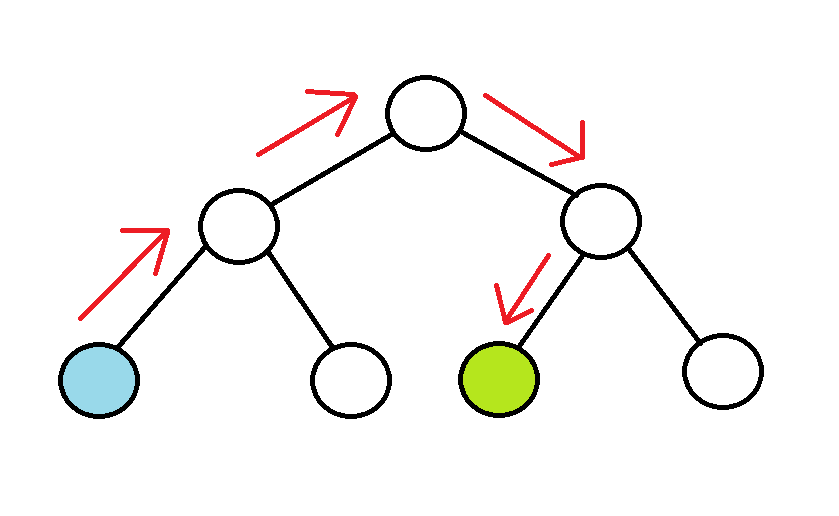
\includegraphics[scale = 0.3]{treeeb.png}
        \caption{distance when common ancestor is 2 levels above = 4}
        \label{fig:2}
        \end{figure}
\end{itemize}

In short, we can conclude,
\begin{align}
    d = 2 * l
\end{align}
where d is the distance between the 2 nodes
\\
l is the number of levels between the leafnodes and their common ancestor.
\subsection{Implementation}
Below is the code for calculating distance between 2 given nodes.
\begin{lstlisting}
https://github.com/hellblazer1/EE4013_A1/tree/main/codes/bar_func.c
\end{lstlisting}
\section{Expected Distance}
Expected distance is given by
\begin{align}
    d = \sum_{n} x.p_X(x)
\end{align}
We can select 2 leaf nodes among 8(repetitions included) in 8x8 ways = 64 ways. Thus, n = 64
\\
Since the nodes are chosen uniformly at random, probability of choosing a pair is $ \frac{1}{64}$. Thus the equation modifies to:
\begin{align}
    d = \frac{1}{64} \sum_{n} x
\end{align}
The summation represents the sum of distances between all possible combinations of leaf nodes. If the pair of leaf nodes contain the same node, then the distance is taken to be 0.

\subsection{Solution}
Below is the code for calculating expected distance.
\begin{lstlisting}
https://github.com/hellblazer1/EE4013_A1/tree/main/codes/bar_func.c
\end{lstlisting}

We get the total distance as 272. Expected length = 4.25


\end{document}
